\documentclass[psfig,preprint]{aastex}
                                                                                
\begin{document}
                                                                                
\title{DOES EVERYTHING WORK PROPERLY? \\
DO THESE CHECKS ON EVERY DAY'S DATA!!}

\author{Carl Heiles (\today)}

\tableofcontents

\clearpage

\section{INTRODUCTION: SOME PROBLEMS WE HAVE EXPERIENCED}

	The problems that we {\it know} of include:
\begin{enumerate}

	\item Dead receivers.

	\item Cables interchanged.  For example, two receivers are
interchanged so that the one that is supposed to be on feed 4, pol B is
really on feed 6, pol B and vice-versa. 

	\item SJU airport radar with a period of
12.0 seconds.  Normally this is not a problem, but when commensally
observing with some extragalactic observers who center at 1385 MHz there
is an intermodulation product that appears in our science band spectrum.
We can get rid of it by changing the \verb$digitalmix$, i.e.\ the 3rd
local oscillator which resides digitally within GALSPECT.

	\item Other radar. There might be periodic signals from other
radar.

	\item Baseline ripple from reflections in the optical fiber.
\end{enumerate}

	The problems that we {\it haven't} experienced\dots well, we
can't tell you about them.  But looking at our diagnostics might reveal
new ones! We have developed software that produces and displays several
diagnostics to easily check for these effects.  These are based on
statistical properties of the non-calibration spectra that reside in
each fits file.  Therefore, there is one set of diagnostics for each
fits file.  Typically you have perhaps a dozen fits files in one day's
observing, so this means you have 12 sets of diagnostics to examine. 

	For a single day's observation the examination process consists
of either printed or plotted output.  (Printed output is not yet
implemented).  We recommend looking at each day's data soon after the
observing period is finished. 

	You should also look at all of your days in combination, because
you can then see trends that are not easily visible on a given day. The
plotted output is better for this because there are too many numbers to
look at on a printed page.

\section{BEFORE WE BEGIN\dots GENERATE THE AUXILIARY FILES CALLED $mh$
AND $lsfs$ FILES}

	For each fits file generated by the GALFA spectrometer, we generate
an auxiliary files called a \verb$mh$ file. The \verb$mh$ file is a
highly abbreviated version of the original fits file; the
space-consuming spectral information is removed, and it also contains
the time series of integrated total powers for each spectrum. In
addition, each fits file must be associated with a calibration file,
which allows us to remove the i.f.\ bandpass and generate 
baseline-corrected spectra. These calibration files are called
\verb$lsfs$ files because the calibrations uses the
Least-Squaares-Frequency-Switching procedure. 

	You must generate the \verb$mh$ and \verb$lsfs$ files before
proceeding further. To do this, see the document ``HOW TO GENERATE MH AND
LSFS FILES''. Alternatively, if you are doing conventional basketweave
observations, that pipeline automatically produces the \verb$mh$ and
\verb$lsfs$ files; see the document ``XXXXXXXXXXx''.


\section{NOW WE REALLY BEGIN! LOOKING AT THE DIAGNOSTICS} \label{looking}

	We describe the diagnostics in some detail in \S
\ref{diagnostics}. First we describe how to look at them, because you
might not care about the details. So here we go\dots

\subsection{Generate the list of $mh$ files to examine}

	The diagnostics are parameters that describe each fits file. 
They are derived independently for each file.  Our diagnostic programs
operate on \verb$mh$ files, which are highly abbreviated versions of the
fits files; they are small enough to be read almost instantaneously. 
The \verb$mh$ files are generated in the very first stage of the data
processing and are normally stored in a subdirectory having the name
\verb$projectname/mh$ for basketweave data or perhaps, at Arecibo,
\verb$/share/galfa/mhmx/$.  They contain two structures called \verb$mh$
and \verb$mx$.  The \verb$mx$ structure contains the diagnostic
information. 

	The first thing to do is generate a file containing the list of
the \verb$mh$ files you are interested in.  We'll call this file
\verb$mhfilelist$.  You can generate this file very easily from UNIX
prompt.  For example, suppose you want all of the \verb$mh$ files for
the togs project that reside in a particular subdirectory (which,
at Arecibo, might be \verb$/share/galfa/mhmx/$).  These \verb$mh$ files
have names like \verb$galfa.20051005.togs.0043.mh.sav$. 

	Get into that subdirectory and type the UNIX command \\
\verb$ls -1 *togs*mh.sav > mhfilelist$ \\
This produces the file called \verb$mhfilelist$, which contains
a single column that lists all the togs \verb$mh$ files (without
any subdirectory prefix). 

\subsection{Look for dead receivers} \label{rcvrbad}

	You do this by invoking the IDL procedure \verb$rcvrbad.pro$.
In the subdirectory where the file \verb$mhfilelist$ exists, enter IDL 
and type the command \\
\verb$rcvrbad, '/share/galfa/mhmx/', 'mhfilelist', mxx=mxx$ \\
By doing
this, you invoke the procedure \verb$rcvrbad$ with its two required
inputs, the path to the \verb$mh$ files and the \verb$mh$ file list
itself. Note the quotes: you are using the actual path and file names as
inputs. Alternatively, you could define IDL variables for these and use
those variables as inputs, in which case you would not use the quotes.
Including the \verb$mxx=mxx$ is handy: \verb$mxx$ is the array of all
the \verb$mx$ structures read from the save files, and if you include
this addition of \verb$mxx=mxx$ it won't have to read them
again\footnote{For the IDL'ers among you, we are bringing the $mxx$
array back to the main level so that it is available there.}.

	The program will produce a plot of the rms/mean power (vertical
axis) versus file number for receiver number 0.  The screen will tell
you that you need to hit a typewriter key to see the next receiver.  If
you type `q` the display will stop incrementing to the next receiver. 
If the plot window is too small you can enlarge it with your cursor, or
with IDL's \verb$window$ function, and run the program again. 

\begin{figure}[!h]
\begin{center}
\plottwo{rcvrbad_2.ps}{rcvrbad_3.ps}
%\includegraphics[width=7in]{rcvrbad_3.ps}
\end{center}
\caption{Plots from $rcvrbad$ for two rcvrs, numbers 2 (feed 1, pol A;
left panel) 
and 3 (feed 1, pol B; right panel). Top panels are wb, bottom nb. 
See text in \S \ref{rcvrbad}
for details. \label{rcvrbadps}}
\end{figure}

	Let's take a look at a sample plot output in figure
\ref{rcvrbadps}.  Each panel plots the rms ratio (y-axis) versus index
number for about 3200 \verb$mh$ files; the scale of days on the
right-hand axes show that these cover almost a year's worth of
observing.  The two left panels are for receiver 2 and the right ones
for receiver 3; the top panels are the wideband data and the bottom the
narrowband.  Contrary to what might be your intuition, systematically
{\it small} values of the rms ratio indicate a nonfunctioning
receiver---because the sky produces nonstatistical fluctuations and if
the receiver doesn't see the sky, its rms is smaller. 

	The two receivers look totally different in the index range
$\sim 800$-1900. All of the other receivers look like receiver 2;
receiver 3 is unique in having those small rms ratios. This shows that
receiver 3 was dead during this interval, which corresponds to the
interval about 20 Jun to 29 Aug 2005.

	Note it's the {\it comparison} of one receiver's plot with the other
receivers' plots that counts. 

	You can play with the cursor and compare plot windows by
blinking; see \S \ref{desiderata} for details.  The Julian day increment
(from the earliest file) is plotted in white (on the screen; black in
figure \ref{feedbadps}), with a scale on the right-hand side of the
plot.  If you want to zoom in on a limited range of Julian day
increments, for example from day increments 23 to 78, you can run the
program again with these as a 2-element vector as an additional input: \\
\verb$rcvrbad, '/share/galfa/mhmx/', 'mhfilelist', mxx=mxx, juld=[23,78]$ \\
or you can instead set a range of the plotted MX INDEX
NR to plot: \\ 
\verb$rcvrbad, '/share/galfa/mhmx/', 'mhfilelist', mxx=mxx, mxindx=[600,800]$

	The program also produces a printed output on the screen.  If
its width exceeds your screen's Xwindow width, you can make your Xwindow
wider and rerun the program.  The printed output gives the Julian days
and calendar dates of the first and last plotted files and additional
information on interpretation. 

\subsection{Look at the feed parameters for problems with feeds}
\label{feedbad}

	You do this by invoking the IDL procedure \verb$feedbad.pro$.
You do this in exactly the same way you did above: in the subdirectory 
where the file \verb$togsfilelist$ exists, enter IDL and type the command \\
\verb$feedbad, '/share/galfa/mhmx/', 'mhfilelist', mxx=mxx$ 

	The program will produce a plot of feedbad for all feeds
(different colors, vertical axis) versus file number that is supposed to
make it clear what's going on.  If the plot window is too small you can
enlarge it with your cursor, or with IDL's \verb$window$ function, and
run the program again. 

\begin{figure}[!p]
\begin{center}
\includegraphics[width=7in]{feedbad.ps}
\end{center}
\caption{Sample plot from $feedbad$. Top panel is wb, bottom is nb. 
See text in \S \ref{feedbad}
for details. This needs color for full reproduction. \label{feedbadps}}
\end{figure}

	Figure \ref{feedbadps} shows a sample of the plotted output.
%,and Figure \ref{feedbadprint.ps} shows a sample of the printed output.
The plotted output uses color, so if you print this document on a
non-color printer you lose the color info on the example. 

	Let's take a look at figure \ref{feedbadps}. There are two
panels; the top is for wb, the bottom nb. Each feed is
shown in a different color; for feed 0-7 the colors are [grey, red,
green, blue, cyan, magenta, yellow]. In each panel there are two groups
of points for each feed, one below and one above 0.75 on the left-hand
vertical scale. A point below 0.75 means that the diagnostic considers the
feed as OK, while above 0.75 there is a problem. The diagnotsic isn't
perfect, so you should look for systematic patterns. Look at MX INDEX
NUMBER $\sim 220$-$630$: you see a solid group of bad points for feeds 4
and 6. These dates correspond to the month of May 2005, when the cables
for pol B of those feeds were interchanged. You also see a solid group
of bad points for feed 1 for MX INDEX NUMBER $\gtrsim 800$. This feed is
bad because one of its receivers was dead. 

		You can play with the cursor and compare plot windows by
blinking; see \S \ref{desiderata} for details.  The Julian day increment
(from the earliest file) is plotted in
white (on the screen; black in figure \ref{feedbadps}), with a scale 
on the right-hand side of the plot. If you want to
zoom in on a limited range of Julian day increments, for example from
day increments 23 to 78, you can run the program again with these as a
2-element vector as an additional input: \\
\verb$feedbad, '/share/galfa/mhmx/', 'mhfilelist', mxx=mxx, juld=[23,78]$ \\
or you can instead set a range of the plotted MX INDEX NR to plot: \\
\verb$feedbad, '/share/galfa/mhmx/', 'mhfilelist', mxx=mxx, mxindx=[600,800]$ 

	The program also produces a printed output on the screen. If its
width exceeds your screen's Xwindow width, you can make your Xwindow
wider and rerun the program. The printed output gives the Julian days
and calendar dates of the first and last files and additional information
on interpretation. 

\subsection{Look for the SJU airport radar} \label{sjubad}

	You do this by invoking the IDL procedure \verb$sjubad.pro$.
In the subdirectory where the file \verb$togsfilelist$ exists, enter IDL 
and type the command \\
\verb$sjubad, '/share/galfa/mhmx/', 'mhfilelist', mxx=mxx$ 

\begin{figure}[!h]
\begin{center}
\includegraphics[height=5in,width=7in]{sjubad.ps}
\end{center}
\caption{Plots from $sjubad$ for two receiver 2. 
Top panel is wb, bottom nb. See text in \S \ref{sjubad}
for details. \label{sjubadps}}
\end{figure}

	The program will produce a plot of the 12-second convolved
power/mean power (vertical axis) versus file number for receiver number
0.  The screen will tell you that you need to hit a typewriter key to
see the next receiver.  If you type `q` the display will stop
incrementing to the next receiver.  If the plot window is too small you
can enlarge it with your cursor, or with IDL's \verb$window$ function,
and run the program again. 

	Let's take a look at a sample plot output in figure
\ref{sjubadps}.  Each panel plots the mean SJU radar power (y-axis)
versus index number for about 3200 \verb$mh$ files; the scale of days on
the right-hand axes show that these cover almost a year's worth of
observing.  The top panels are the wideband data and the bottom the
narrowband. 

	You see two groups of points, one with positive amplitude and
one with negative.  (Ignore the zero points---they have no cal-off
data).  The negative group gives an impression of what to expect from
random noise.  The larger number of positive points shows that we have radar
leaking in.  These points are derived from total power, not spectral
features, and what is most likely happening is the SJU radar changes the
total system level without introducing noticeable spectral
features---unless intermodulation products are at work. 

	Note the change in in appearance beginning at MX INDEX NUMBER
$\sim 1900$. This occurs because most of those files are from the
\verb$togs$ program, which piggybacks on the ALFALFA group. They set the
first l.o.\ lower than GALFA observers do, so the SJU radar leaks into
our wideband spectra. This produces saturation during those times when
the SJU radar pulse is on, and this is reflected in figure
\ref{sjubadps}. 

	The SJU plots like figure \ref{sjubadps} reflect the {\it
overall continuum level} but don't tell much about {\it spectral
features}.  For example, from MX INDEX NUMBER $\sim 1900$ to 2540, we
had an intermodulation product from the SJU radar in our science band,
which produced a fake HI line (usually at the few-tenths K level, but
sometimes much stronger).  On 12 September (indx $\sim 2540$) we changed
our second and third l.o.\ (the third l.o.\ is controlled by
\verb$digitalmix$), which placed the intermodulation product outside of
the narrow band.  This is not reflected in the continuum plot of figure
\ref{sjubadps}.  To see such spectral contamination you need to look at
{\it spectra}.  We illustrate this process in \S \ref{quickfile}, below. 

		You can play with the cursor and compare plot windows by
blinking; see \S \ref{desiderata} for details.  
The Julian day increment (from the earliest file) is plotted in
red, with a scale on the right-hand side of the plot. If you want to
zoom in on a limited range of Julian day increments, for example from
day increments 23 to 78, you can run the program again with these as a
2-element vector as an additional input: \\
\verb$sjubad, '/share/galfa/mhmx/', 'mhfilelist', mxx=mxx, juld=[23,78]$ \\
or you can instead set a range of the plotted MX INDEX NR to plot: \\
\verb$sjubad, '/share/galfa/mhmx/', 'mhfilelist', mxx=mxx, mxindx=[600,800]$ 

	The program also produces a printed output on the screen. If its
width exceeds your screen's Xwindow width, you can make your Xwindow
wider and rerun the program. The printed output gives the Julian days
and calendar dates of the first and last files and additional information
on interpretation. 

\subsection{Look for periodic signals such as radars with arbitrary periods}
\label{radarbad}

	You do this by invoking the IDL procedure \verb$radar.pro$.
In the subdirectory where the file \verb$togsfilelist$ exists, enter IDL 
and type the command \\
\verb$radarbad, '/share/galfa/mhmx/', 'mhfilelist', mxx=mxx$ 

\begin{figure}[!h]
\begin{center}
\includegraphics[height=5in,width=7in]{radarbad.ps}
\end{center}
\caption{Plots from $radarbad$ for receiver 1. 
Top panel is wb, bottom nb. See text in \S \ref{radarbad}
for details. \label{radarbadps}}
\end{figure}

	The program will produce a plot of the strongest radar period
(vertical axis) versus file number for receiver number 0; the amplitude
of the strongest radar signal is indicated by the size of the plot
symbol.  The screen will tell you that you need to hit a typewriter key
to see the next receiver.  If you type `q` the display will stop
incrementing to the next receiver.  If the plot window is too small you
can enlarge it with your cursor, or with IDL's \verb$window$ function,
and run the program again. 

	Let's take a look at a sample plot output in figure
\ref{radarbadps}.  Each panel plots the period of the strongest periodic
signal versus index number for about 3200 \verb$mh$ files; the scale of
days on the right-hand axes show that these cover almost a year's worth
of observing.  The top panels are the wideband data and the bottom the
narrowband. 

	Each point has a period and a power. The size of the point is
proportional to the power, up to a limit---bigger points, more power.
Most small points are meaningless random noise. Most prominent are the
rows of large points with periods of 6 and 12 seconds. We suspect that
the 6-second points are really 12 second points, because we derive the
periods by looking in the frequency (not period) domain and allowing for
subharmonics. 12 second corresponds to the SJU radar. We don't see any
other prominent, systematic periods.

	As with the SJU radar plots of \S \ref{sjubad}, these reflect
the {\it overall continuum level} but don't tell much about {\it
spectral features}.  For example, from MX INDEX NUMBER $\sim 1900$ to
2540, we had an intermodulation product from the SJU radar in our
science band, which produced a fake HI line at the few-tenths K (or
sometimes much more) level.  On 12 September (indx $\sim 2540$) we
changed our second and third l.o.\ (the third l.o.\ is controlled by
\verb$digitalmix$), which placed the intermodulation product outside of
the narrow band.  This is not reflected in the continuum plot of figure
\ref{sjubad}.  To see such spectral contamination you need to look at
{\it spectra}.  We illustrate this process in \S \ref{quickfile}, below. 

		You can play with the cursor and compare plot windows by
blinking; see \S \ref{desiderata} for details.  
The Julian day increment (from the earliest file) is plotted in
red, with a scale on the right-hand side of the plot. If you want to
zoom in on a limited range of Julian day increments, for example from
day increments 23 to 78, you can run the program again with these as a
2-element vector as an additional input: \\
\verb$radarbad, '/share/galfa/mhmx/', 'mhfilelist', mxx=mxx, juld=[23,78]$ \\
or you can instead set a range of the plotted MX INDEX NR to plot: \\
\verb$radarbad, '/share/galfa/mhmx/', 'mhfilelist', mxx=mxx, mxindx=[600,800]$ 

	The program also produces a printed output on the screen. If its
width exceeds your screen's Xwindow width, you can make your Xwindow
wider and rerun the program. The printed output gives the Julian days
and calendar dates of the first and last files and additional information
on interpretation. 

\subsection{A little different: look at SPECTRA!} \label{quickfile}

	This diagnostic differs from the above four.  In those, you
averaged over {\it frequency} (integrated over the whole bandpass) and
statistically analyzed the {\it time} series.  Here, we average over {\it
time} and let your eye analyze the {\it frequency} spectra. This allows
you to see the effects of radar. Also, there is usually some ripple in
the spectra (period $\sim 200$ kHz), which results from reflections in
the optical fibers that bring the signal from the feed to the control
room (see \S \ref{desiderata}).

	We examine each fits file independently, as we did above.  We
calibrate the spectra in approximately the same way as we do for the
final data product (only the intensity scales differ, and not by more
than perhaps $10\%$).  For each fits file we find all the spectra not
used for calibration; presumably, what remains is ordinary data used for
your observing program.  We calibrate these non-cal spectra individually
and average them.  The calibration process is time consuming, so we save
the results in ``quick'' files having the suffix \verb$qck.sav$; at
Arecibo we currently store them in subdirectory \verb$/share/galfa/qck/$. 
Then we use different program to plot the results. 

	So it's a two-stage process. First you generate the quickfiles;
then you look at them. 

\subsubsection{Generate the quickfile} 

	Generating the quickfiles requires calibrating the data, which
in turns needs the \verb$lsfs$ files, so you have to first generate
these.  At the moment the process of generating the quickfiles requires
you choosing an \verb$lsfs$ file for each \verb$fits$ file you treat. 
This is an annoying necessity and we will automate this choice someday. 

	You first need to specify the various paths.  These include the
path to the fits file \verb$fitspath$, the path to the lsfs file
\verb$lsfspath$, the path where to write the quickfile \verb$qckpath$,
the name of the \verb$fitsfile$ you want to process, and the name of the
\verb$lsfsfile$ you associate with the \verb$fitsfile$.  
It's convenient to define these variables in IDL so you can call the
procedure with variable names instead of strings.  An example that works
for Arecibo is \\
\verb$fitspath = '/share/galfa/'$ \\
\verb$lsfspath= '/share/galfa/lsfs_carl/'$ \\
\verb$qckpath=  '/share/galfa/qck/'$ \\
\verb$lsfsfile= 'lsfs.20050905.1125996998.togs.0065.sav'$ \\
\verb$fitsfile= 'galfa.20050905.togs.0056.fits'$ 

	Then, to make the file, you invoke the procedure
\verb$simpred_ch$: \\ 
\verb$simpred_ch, fitspath, lsfspath, fitsfile, lsfsfile, qckpath, qckfile$ \\
	Note: \verb$qckfile$ is an {\it output}: you don't specify its
name because it's generated automatically, and the name \verb$qckfile$
contains the path so that you can use this as a single variable to read the 
quickfile. Also, note that
\verb$fitsfile$ is not a list, it's the name of an individual file. This
progam does one fits file at a time; if you want to process several, you
can use a \verb$for$ loop. 

\subsubsection{Looking at the quickfile}

	This is easy. You know the name and path to the quickfile---it's
\verb$qckfile$ from immediately above. Or, if you are looking at some
arbitrary quickfile whose name is, for example,
\verb$galfa.20050905.togs.0056.qck.sav$ which resides in
\verb$/share/galfa/qck/$ (which you previously defined as \verb$qckpath$), 
define the variable \verb$qckfile$ yourself: \\
\verb$qckfile = qckpath + 'galfa.20050905.togs.0056.qck.sav'$ \\
or equivalently
\verb$qckfile = '/share/galfa/qck/', 'galfa.20050905.togs.0056.qck.sav'$ 

\begin{figure}[!h]
\begin{center}
%\includegraphics[height=5in,width=7in]{radarbad.ps}
\includegraphics[height=5in,width=7.in]{quickplot.ps}
\end{center}
\caption{Plots from $quickplot$. 
Left panel is wb, right nb. See text in \S \ref{quickfile}
\label{quickplotps}}
\end{figure}

	Having done this, generate the plot with \\
\verb$quickplot, qckfile$ \\
This procedure plots all 14 spectra, one above the other, offset by
\verb$dely=1.5$ K; see the example in figure \ref{quickplotps}. The parameter
\verb$dely$ also sets the plot scale.  
\verb$dely=1.5$ K is the default values; you can change it when you invoke the
procedure, for example \\
\verb$quickplot, qckfile, dely=2$ 
	
	In figure \ref{quickplotps} there are 15 plots, not 14. The top
one (in red if you have a color printout) is the average of the 14
receivers. The receiver number increases sequentially from 0 to 13 going
{\it up} the page. The bottom two, rcvrs 0 and 1, are pols A and B on
feed 0, etc. 

	Note the wiggles on the wb and nb spectra.  These wiggles are
not thermal noise.  Rather, they are ``fixed-pattern'' noise: the
pattern repeats from day to day.  Some of its statistical properties are
discussed in the memo ``SOME CHARACTERISTICS OF ALFA'S FIXED PATTERN
NOISE (FPN)''.  We're pretty sure that this fixed pattern noise is also
present on the LBW receiver. We are currently trying to understand its
origins with the aim of reducing it. 

	There is also a printout, two columns of temperatures, which
are the spectrum-averaged powers (in K) before baseline subtraction. And
there is a test for whether the lo frequency of the LSFS calibration was
significantly different from that of the observed spectra; a bunch of
stars are printed and a warning message issued if this is the case. If
it {\it is} the case, it's not necessarily serious because the LSFS is used
to determine the i.f.\ bandpass shape, which should be independent of
l.o.\ frequency.

\subsection{Desiderata}
\label{desiderata}

	In this section we provide some hints and comments on extracting
info from your plots.  These including using a cursor, finding the fits
filename that goes with a particular datapoint, and getting rid of the
i.f.\ ripple. 

\subsubsection{Using the cursor}

	If you want to pinpoint a particular datapoint you want to use
the cursor.  To do this, get to the IDL prompt.  You might be there
already, but if you are cycling through receivers you will need to type
CTRL-C.  From the IDL prompt, type \verb$trc$ and move the cursor to the
plot window.  Only the most recent plot will display the green cursor
lines.  Put the cursor over the point of interest and press the lefthand
mouse button; the coordinates are written on the screen.  You can do
this again and again.  When you are tired of this game, press the
righthand mouse button, which gives you back the prompt. If you are
stopped in the middle of some procedure aand want to continue, type
\verb$.cont$ . 

\subsubsection{Blinking two plots}

	Suppose you are cycling through the receivers and want to blink
two of those plots. The procedure is: first blink one plot against
itself and make a copy of the blinked result; then blink the second one
against that copy. To accomplish this, while cycling through the
receivers type CTRL-C before the one you want to blink. Suppose you are
looking at plots in window 1. Then type \\
\verb$cblink,[1,1]$ \\
which will blink window 1 against itself (i.e., no blinking!) and stop it by
hitting a key other than ``d'' (See the instructions on the screen). 
It will store the original window into
another one, and it will tell you the new one's number, which will
probably be number 32. Then type \verb$.cont$ to get the
receiver plotting again. Hit CTRL-C before the second receiver you want
to blink, which again gives you the IDL prompt. Now type \\
\verb$cblink,[1,32]$ \\
to blink the two windows against each other.

\subsubsection{How do I determine which file goes with which data?}

	For the first four diagnostics you have plots versus MX INDEX
NUMBER.  First, use the cursor to get the MX INDEX NUMBER.  For any
INDEX NUMBER (for example, 1803) you can determine the associated fits
file name by typing the IDL command \\ 
\verb$print, mxx[1803].fitsfilename$

\subsubsection{The i.f.\ ripple}

	The optical fibers that bring the signal down to the control
room can have reflections at the ends if they are not properly matched. 
This produces a ripple in the narrowband spectra with a period of
roughly 200 kHz.  You can see this on the spectral plots of figure \ref
{quickplotps} in \S \ref{quickfile}. 

	It's great to see it, but what do you do about it? You can use
the program \verb$zapft$; you can get it's documentation by entering IDL
and doing the usual thing for well-documented procedures, namely type \\
\verb$doc_library, 'zapft'$

You'll see it wants inputs \verb$frqin, ydata, degree$. The program fits
a combination of a polynomial and a single Fourier component;
\verb$degree$ specifies the degree of the polynomial, which should
normally be zero. \verb$ydata$ is the 7679-point spectrum. \verb$frqin$
is the set of baseband or i.f.\ frequencies associated with the
spectrum; an acceptable array\footnote{Brief explanation of this
equation: the narrowband bandwidth is $100 \over 14$ MHz. Originally
there area 8192 channels, of which we retain only 7679. The $d$ suffix
means ``double precision''.} to use is 
given by the IDL command \\
\verb$frqin= (dindgen( 7679) - 7679.d/2.d)* 100.d/(14.*8192.)$

	We have little experience using \verb$zapft$. It works well when
the ripple is strong enough to see. This is usually the case only on a
bunch of spectra averaged together. We don't know if it works on a
single one-second spectrum. If you experiment with this, please let us
know what you find.

\section{DIAGNOSTICS IN DETAIL} \label{diagnostics}

	There are five diagnostics for each fits file.  Four are arrays
that are in an IDL structure called \verb$mx$ which is recorded in the
\verb$mh$ files.  The fifth is the average of all non-cal spectra within
the fits file.  These are in ``quickfiles''; at Arecibo, these probably
reside in the subdirectory \verb$/share/galfa/qck$.  Here are the first
four diagnostics, called by their variable names in the software:
\begin{enumerate}

	\item To indicate interchanged receiver cables between feeds we
crosscorrelate each receiver's power time series with every other
receiver' series and generate the $14 \times 14$ crosscorrelation
matrix.  This process uses a highly filtered version of the 14
receivers' time series.  We then examine this matrix to create the
7-element integer arrays \verb$m1.feedbadwb$ and \verb$m1.feedbadnb$ for
the wideband and narrowband spectra, respectively---one array element
for each beam.  The elements of these arrays are zero unless there is an
indication of interchanged cables, in which case the affected elements
are 1. 

	For example, in the past, receivers to feeds 4 and 6 were
interchanged, so we should have these arrays equal to
\verb$m1.feedbadwb=[0,0,0,0,1,0,1]$ (ditto for \verb$m1.feedbadnb$). 
That is, feeds affected by interchanged cables should come in pairs! In
practice, for these data we had \verb$m1.feedbadwb=[0,1,0,0,1,0,1]$
because one of the receivers on feed 1 was bad.  We knew this from
looking at the receiver diagnostic. 

	\item To indicate a dead receiver we take each receiver's power
time series, take its rms, and divide it by its mean.  If there were
nothing other than thermal noise, this ratio would be the reciprocal of
the square root of the time-bandwidth product for the 1-second
integrations.  In fact, there are gain variations and continuum sources
moving through the beam, so the ratio is much larger. An anomalously
small ratio means that the receiver isn't working. We look at the set of
14 ratios and declare any receiver bad whose ratio is half the global
median of the 14 ratios. 

	We report the results in the 14-element integer arrays
\verb$m1.rxbadwb$ and \verb$m1.rxbadnb$ for the wideband and narrowband
spectra, respectively. The elements are zero unless the rms ratio is out
of bounds, in which case the corresponding element is unity. 

	\item The San Juan radar has a 12 second periodicity.  We look
for this taking each receiver's power time series, producing a highly
filtered version to eliminate non-radar interference spikes, and
crosscorrelating with a pulse train having 12 second period.  We record
the largest value of this 12-point crosscorrelation function, divided by
the mean power in the time series, in the 14-element arrays called
\verb$mw.sjuwb$ and \verb$m2.sjunb$ for the wideband and narrowband
spectra, respectively.  Large values (we don't really know yet what
``large'' means) indicate a SJU radar problem.  Negative values are
probably statistical fluctuations on nearly radar-free data. 

	\item Maybe there are other radars affecting your data! To check,
we take each receiver's power time series.  We produce a highly filtered
version to eliminate slow drifts and non-radar interference spikes.  We
take the autocorrelation function and then Fourier transform it to look
for spectral peaks.  We check for subharmonics in the peaks and pick the
largest amplitude one and report the result in the $2 \times 14$ element
arrays \verb$mx.rxradarwb$ and \verb$mx.rxradarnb$.  There are two
elements for each receiver.  The first is the period in seconds and the
second is the power in that Fourier component divided by the mean power. 

\end{enumerate}

	The above four diagnostics are statistical in nature.  We have a
fifth diagnostic, which is the shape of the spectrum averaged over the
fits file.  We exclude 1-second contributions that were used for
calibration, meaning spectra labeled as SMARTF or those taken with the
cal on.  These averaged spectra are corrected for bandpass and are
baseline-subtracted in the same way as the final spectra are.  Their
intensities are in approximate Kelvins ($\sim 20\%$ accuracy).  These
spectra can only be generated after the \verb$mh$ files are generated so
they are written out in separate files with a \verb$qck.sav$ suffix,
e.g.\ \verb$galfa.20050905.togs.0056.qck.sav$ in the subdirectory
\verb$/share/galfa/qck/$. 

\acknowledgements

        This research was supported in part by NSF grant AST 04-06987    
and by the NAIC.

\end{document}
		
